\section{Methodology}\label{sec:methodology}
Given the absence of a library adoption model in the literature, we decided to adopt Straussian grounded theory \cite{corbin2014gt} to derive such a model.  
% All of the authors of this paper have at least ten years of industry experience. As such, it was also important that our formulation of the library adoption model is derived from the responses of study participants, while the model is not biased by our prior own experience. 
% Unlike classical grounded theory, Straussian grounded theory acknowledges the presence of research bias, assumptions, and motivations, and provides structured tools (constant comparison and memoing) to handle the intrusion \cite{stol2016grounded,corbin2014gt}. 
We chose to conduct semi-structured interviews of industry developers to learn about the model because such interviews allow us to elicit unexpected information and to evolve our questions as the study progresses \cite{HoveAnda, Seaman}. 
Figure~\ref{fig:methodology} provides an overview of the overall research method which was applied to the study.
\begin{figure*}
    \centering
    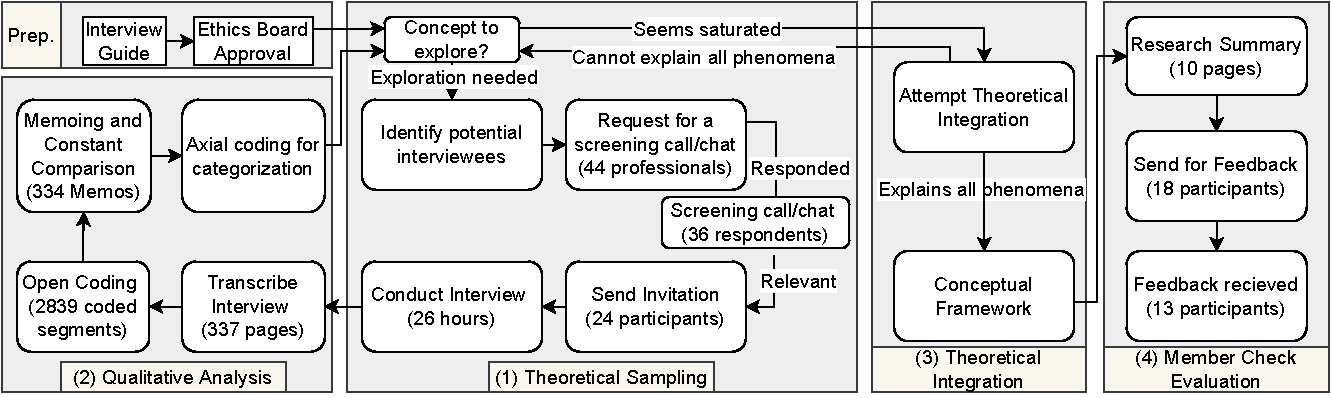
\includegraphics[scale=.7]{images/methodology.pdf}
    \caption{Grounded theory research method applied}
    \label{fig:methodology}
\end{figure*}



% Because the study involved human subjects, we obtained approval from the Ethical Review Board of our institution before conducting interviews. In total, we conducted \numInterviews interviews, interleaving data collection and analysis following grounded theory design principles. Figure~1 in the Appendix shows the overall research process.




% \begin{table*}[]
%     \centering
%     \begin{tabular}{p{.4cm}r{.4cm}l{2.5cm}l{2cm}l{2cm}l{2.2cm}r{2cm}r{1.5cm}}%{lrllllrr}
% \toprule
% P\# & Yrs & Role & Primary Tech & Continent & Industry & Company Size & Tech Size \\
%     \midrule
% P1 & 12 & Architect & Java & Europe & Automotive & 4000 & 500 &  \\ 
% P2 & 6 & Software Engineer & Python & North America & Cloud Service & 150000 & 80000 &  \\ 
% P3 & 12 & Software Engineer & Android+iOS & North America & Automotive & 30000 & 600 &  \\ 
% P4 & 20 & CEO & .NET, AWS & Asia & Broadcast Media & 60 & 54 &  \\ 
% P5 & 16 & Engr. Manager & .NET, AWS & Australia & Financial & 40 & 12 &  \\ 
% P6 & 17 & Software Engineer & Perl & Europe & Tech & 200 & 20 &  \\ 
% P7 & 9 & CTO & Javascript & North America & Data Analytics & 21 & 6 &  \\ 
% P8 & 9 & Software Engineer & Any Tech & North America & Cloud Service & 20000 & 10000 &  \\ 
% P9 & 13 & Architect & Python & North America & Web & 250 & 100 &  \\ 
% P10 & 15 & Software Engineer & Javascript & Europe & Energy & 11000 & 300 &  \\ 
% P11 & 7 & ML Engineer & Python & North America & Data Analytics & 100 & 30 &  \\ 
% P12 & 22 & Consultant & Perl & Asia & Tech & 30000 & 1000 &  \\ 
% P13 & 15 & Architect & Java & North America & Retail & 1000000 & 200000 &  \\ 
% P14 & 6 & Software Engineer & Android+iOS & Asia & Financial & 150 & 100 &  \\ 
% P15 & 22 & CTO & .Net & Asia & Enterprise & 350 & 300 &  \\ 
% P16 & 9 & Software Engineer & Java & Asia & Cyber Security & 400 & 300 &  \\ 
% P17 & 15 & CTO & Ruby on Rails & Europe & Custom Software & 35 & 6 &  \\ 
% P18 & 27 & CEO & C++ & North America & Financial & 150 & 40 &  \\ 
% P19 & 15 & Engr. Manager & Ruby on Rails & North America & Cloud Service & 150000 & 75000 &  \\ 
% P20 & 10 & Software Engineer & Android+iOS & North America & Food Service & 70 & 10 &  \\ 
% P21 & 13 & Software Engineer & Ruby on Rails & North America & CI/CD & 1800 & 900 &  \\ 
% P22 & 30 & Architect & Java & North America & Operating Sys. & 19000 & 9000 &  \\ 
% P23 & 7 & ML Engineer & Python & South America & Custom Software & 900 & 750 &  \\ 
% P24 & 6 & ML Engineer & Python & North America & Medical & 150 & 80 &  \\ 

%     \bottomrule
%     \end{tabular}
%     \caption{Interview participant's Professional profile along with the industry and size of their companies}
%     \label{tab:participants}
% \end{table*}


\begin{table}[]
    \centering
    \begin{tabular}{p{.4cm}p{.4cm}p{.5cm}p{.8cm}p{.5cm}p{2.2cm}r{.5cm}}%{lrllllr}
\toprule
P\# & Yrs & Role & Tech & GEO & Industry & Tech Size \\
\midrule
P01 & 12 & Arc & JV & EU & Automotive & 500 &  \\ 
P02 & 6 & SDE & PY & NA & Cloud Service & 80,000 &  \\ 
P03 & 12 & SDE & A/IOS & NA & Automotive & 600 &  \\ 
P04 & 20 & CEO & .NET & AS & Broadcast Media & 54 &  \\ 
P05 & 16 & EM & .NET & AU & Financial & 12 &  \\ 
P06 & 17 & SDE & PE & EU & Tech & 20 &  \\ 
P07 & 9 & CTO & JS & NA & Data Analytics & 6 &  \\ 
P08 & 9 & EM & Any & NA & Cloud Service & 10,000 &  \\ 
P09 & 13 & Arc & PY & NA & Web & 100 &  \\ 
P10 & 15 & EM & JS & EU & Energy & 300 &  \\ 
P11 & 7 & MLE & PY & NA & Data Analytics & 30 &  \\ 
P12 & 22 & Cons & PE & AS & Tech & 1,000 &  \\ 
P13 & 15 & Arc & JV & NA & Retail & 200,000 &  \\ 
P14 & 6 & SDE & A/IOS & AS & Financial & 100 &  \\ 
P15 & 22 & CTO & .NET & AS & Enterprise & 300 &  \\ 
P16 & 9 & SDE & JV & AS & Cyber Security & 300 &  \\ 
P17 & 15 & CTO & RoR & EU & Custom Software & 6 &  \\ 
P18 & 27 & CEO & C++ & NA & Financial & 40 &  \\ 
P19 & 15 & EM & RoR & NA & Cloud Service & 75,000 &  \\ 
P20 & 10 & SDE & A/IOS & NA & Food Service & 10 &  \\ 
P21 & 13 & SDE & RoR & NA & CI/CD & 900 &  \\ 
P22 & 30 & Arc & JV & NA & Operating Sys. & 9,000 &  \\ 
P23 & 7 & MLE & PY & SA & Custom Software & 750 &  \\ 
P24 & 6 & MLE & PY & NA & Medical & 80 &  \\ 

    \bottomrule
    \end{tabular}
    \caption{Interview participants by years in industry, role (Arc-Architect, EM-Engineering Manager, Cons-Consultant, SDE-Software Development Engineer, MLE-Machine Learning Engineer, CTO-Chief Technology Officer), primary technology (JV-Java, PY-Python, A/IOS-Android/iOS, PE-Perl, JS-JavaScript, RoR-Ruby on Rails, Any-not limited by technology) geographic location (AS-Asia, AU-Australia, EU-Europe, NA-North America, SA-South America), industry, and company tech size.}
    \label{tab:interviewee-profile}
\end{table}

\subsection{Participant Recruitment Strategy}
We conducted \numInterviews interviews between June 2022 and January 2023. Table~\ref{tab:interviewee-profile} provides an overview of participants.
The average number of years of professional experience of the participants was 14 years. Their roles spread across the spectrum of engineering and leadership roles and in nine different countries from five continents. The tech stack also had wide varieties (e.g., C/C++, Java, Python, Android, iOS, .NET, machine learning, etc.). Many of our participants were working in large corporations (e.g., Google, Microsoft, etc.) and open-source projects. Among all the interviewees, three experts identified themselves as female. Our participants covered 16 application domains including specialized regulated areas as such health, finance, cybersecurity, and broadcast media. 

 % An important part of grounded theory is theoretical sampling of the concepts. It means that after every interview, we had to perform data analysis of the interview, identify the concepts which needed further elaboration, and select the next few interviewees to improve the probability of getting answers regarding emerging concepts. Before conducting interviews, we performed initial screening of the participants through a short phone call (around 5 to 10 minutes). After we identified that a participant could provide relevant insights, we sent them a formal interview invitation. 
 % In this way, we reached out to 38 potential participants for initial screening of emerging concepts through the professional network of the authors. 



\subsubsection{Theoretical Sampling for Recruitment}
\begin{table*}[]
    \centering
    \begin{tabular}{p{.4cm}p{4cm}p{6cm}p{6cm}}%{llll}
    \toprule
    P\# & Concept we wanted to enhance & Why we selected this Participant & Concepts they enriched significantly \\ 
    \midrule
P1 & Initial process and factors & Architect of a large system & Library definition, factors, influences \\ 
P2 & Licensing and Security Issues & Working in a large structured company & License, company technology \\ 
P3 & Mobile development Factors & 12+ years experienced in mobile application & Cost, company tech, comparison  \\ 
P4 & Long term maintenance concerns & Being a CEO, takes decisions considering long term impact & Company application domain, active development of library \\ 
P5 & Decision making processes & Stablishing the processes in a startup team & Information search, company culture \\ 
P6 & Open Source factors & Has experience regarding OSS contribution and research & Open source, Personal motivation \\ 
P7 & Factors for a startup & Being a startup CTO may share different priorities & Flexibility, Ease of Installation, Community Support \\ 
P8 & Performance factors & Working in a cloud company that may requiew high performing libraries & Familiarity, Team Discussion, Library Migration \\ 
P9 & Migration scenarios & Experienced to migrate company tech stack as architect & Legal risks, Lack of Stability, Less prefered than native support \\ 
P10 & Visualization and front end libraries & Working as web developer for over a decade & Customer support, flexibility, existing repository \\ 
P11 & Machine learning libraries & Experienced in machine learning in gradudate research studies and in industry & Talk to people, Performance, Outstanding library selection \\ 
P12* & DevOps Process for Library Security Issues & Consulted dozens of companies in DevOps process establishment & Barriers of library usage, Baggage of libraries \\ 
P13 & Selection process in large organizations for legal and security risks & Has been an architect in a large team for 10+ years & Consent Process, Benefits of libraries, Tech Expert Opinion \\ 
P14 & Library migration scenarios & Experienced in managing mobile apps with large user base in all platforms & Make life easy, Life long maintenance, Migration to other library \\ 
P15 & Organizational process and motivation for libraries & Experienced in organization process since increased dev team from 3 to 300 & Delivery Deadline, Don't Reinvent the wheel, Feature criticality \\ 
P16* & Process of security concerns & Cerified security professional actively developing security products & License issues, Data Transfer Security, Geographic Impact  \\ 
P17 & Security Process & Delivers custom software to customers and maintains SecOps in CI/CD & Post Integration Maintenance for Security \\ 
P18 & C++ libraries in large scale long term products & Leads development of a 30 year old product written in C++ with 2M lines of code & Lifelong Maintenance Burden, Compatibility, Uniform Coding Style \\ 
P19 & Company Culture, Open Source, Concept Saturation & Experienced working in start-up and large organizations who open source libraries & Standard practices in large organizations, Considerations in open source \\ 
P20 & Challenges in mobile application libraries, Concept Saturation & Full career in mobile app development, mostly in iOS which requires more maintenance & Lifelong Maintenance Burden, Abandoned Libraries, Migration \\ 
P21 & Company Culture, Open Source, Concept Saturation & Works full-time in a prominent open core company & Company policies, Guiding Principles \\ 
P22 & Guiding Principles, Open Source & Experienced in persuing large corporation for open source library adoption & Guiding Principles \\ 
P23 & ML libraries & Working in South America in ML domain & ML Library Dependency Issues \\ 
P24 & Company Culture, Industry, ML Libraries & Working in health sector using ML libraries extensively. & ML Library deployment and upgrade issues \\ 

\bottomrule
    \end{tabular}
    \caption{How we recruited interview participants following theoretical sampling for Concept Saturation. (We could not enhance targeted concepts from the *-marked participants (P12, P16), rather enriched other important concepts.)}
    \label{tab:theoritcal-sampling}
\end{table*}
We started with an architect (participant P1) from our professional acquaintance who had twelve years of experience including designing and developing from scratch a payment system in a 260 human-year project spanning over six years. We knew that they had to select a huge number of libraries throughout this development. Our first interview lasted  115 minutes, as we were developing initial concepts around all of our research questions, while subsequent interviews averaged 64 minutes. % range 42-115
After analyzing the initial interview data, we realized that we needed more information about commercial factors (particularly licensing) and the integration process of a library. Hence, we chose our next participant (P2) who was working in a large organization (\#engineers $\geq$ 80K), and who had experience with licensing concerns about software libraries. In this way, we continued the theoretical sampling to saturate all the relevant concepts. We recruited the interviewees from the direct or extended professional networks of the three authors each of which had more than ten years of software industry experience. Before any interview, we conducted a screening call or email conversation to confirm the relevance of the interviewee regarding the specific concept we wanted to explore. The motivation for selecting every participant is provided in the table \ref{tab:theoritcal-sampling}. 
% In most of the cases, we were able to extract insights about target concept from the interviewees. For example, we wanted to dig deep into the library maintenance issues and we identified mobile applications need continuous update because of the yearly operating system update. Hence we reached out to a mobile developer P14 who actively manages applications in all mobile OS platforms and in the interview, they provided us significant insights about maintenance and migration issues. 


\subsubsection{Concept Saturation over the Interviews}
\begin{figure*}
    \centering
    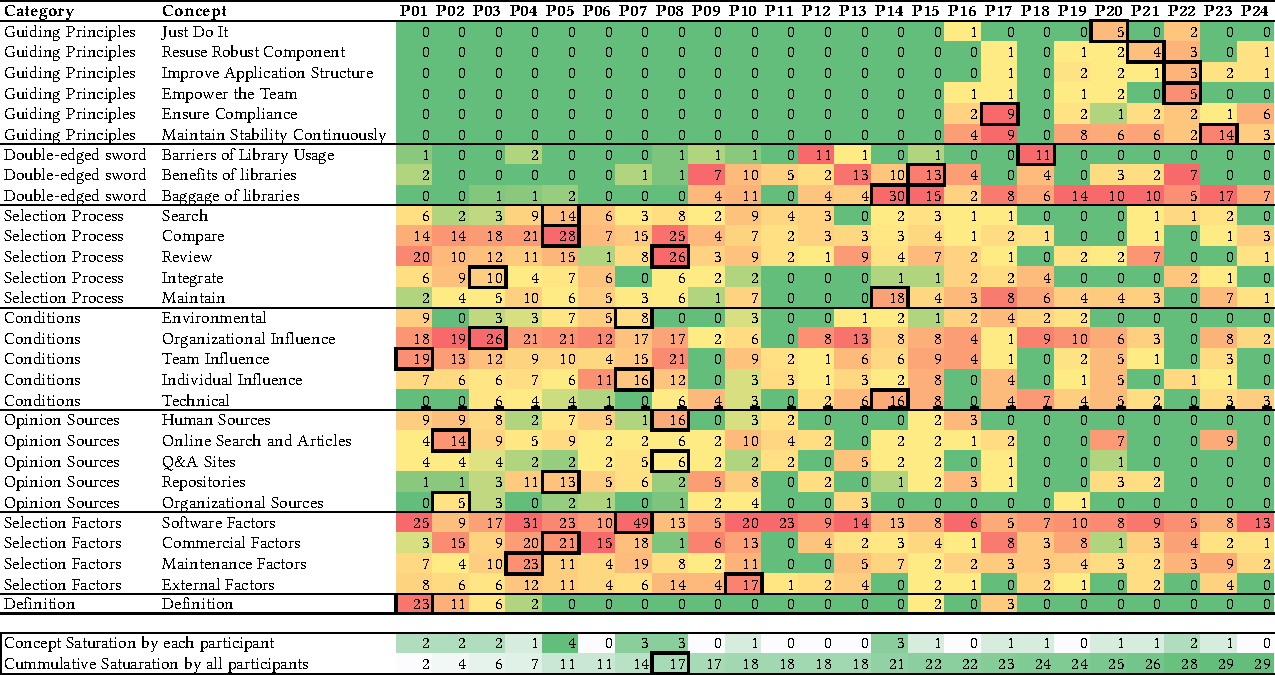
\includegraphics[scale=0.8]{images/saturation.pdf}
    \caption{Heatmap of concept saturation over the interviews. Red refers to higher discussion of a concept by an interviewee, the number refers to how many times interviewee has discussed a concept. Green refers to lower discussion of concepts by an interviewee.}
    \label{fig:saturation}
\end{figure*}
Figure~\ref{fig:saturation} shows how the concepts were discussed during each interview. The number denotes how many times a concept was discussed by one particular interviewee. The more a participant discussed a particular concept, the more red the corresponding cell is. For example, the library search concept was most discussed by P5 (14 times). After their interview, subsequently, we did not have much to discuss the search process, for example, P10 also discussed the same concept 9 times. Hence after we reach a maximum number of times a concept has been discussed, we consider that the concept is saturated. Still, for the sake of a uniform discussion with the interviewees, we keep discussing the concepts in case any new corner case comes up. Whereas library selection factors were saturated by P10 (external factors concept were most discussed by P10 and then gradually declined in consecutive interviews), the conditions and the selection process were saturated by the interview of P14. However, it took us interviews till P18 to attain maximum discussion of barriers to library usage (11 times) and P23 to saturate the concept of maintaining continuous stability. By the time we interviewed P24, no further concepts were discussed and all previous concepts were saturated well beforehand. 

% Our work was initiated with the question RQ1: ``What are the major steps developers follow during their adoption of a software library?'' We soon realized that the process is influenced by certain conditions and factors, leading us to ask RQ2: ``What conditions and technical factors influence the library adoption process?'' 
% %As we continued to conduct interviews, our concepts started to saturate. Though many interviewees contributed towards the saturation, a few interviewees contribute most, and after such an interview a concept saturates very quickly. 
% By time we interviewed P8, we also realized that there were specific library selection principles and many pros and cons of libraries depending on the scenarios. Also after hearing P9's concerns about third-party libraries, we started to discuss about benefits and barriers more. This led to RQ3: ``What guiding principles do developers follow in library adoption?'' These concepts were well understood by the time we interviewed P22. The concepts and principles all saturated by the time we completed our last interview (i.e., P24).

%\textcolor{blue}{[Minaoar]}
%Our work was initiated by the following question: \textit{\textbf{RQ1:} How developers adopt third-party libraries?} After understanding the adoption process, we realized that the process is influenced by certain conditions and technical factors. Then we tried to answer \textit{\textbf{RQ2}: What conditions and technical factors influence the library adoption process?} Finally, we were curious why developers change adoption process based on the conditions and factors? Is there any guiding principles developers follow for library adoption? Then our final question was \textit{\textbf{RQ3:} What guiding principles developers follow in library adoption?} \ab{I'd put this in the methodology where you're talking about GT}

% \subsubsection{Repeated Interviews for Open Questions}
% However, in few cases, we could not find elaboration of our target concept from the interviewee and had to plan for other participants who could answer the questions we had. For example, we expected that P12, who specializes in DevOps process establishment in tech companies, could share experience on continuous monitoring of libraries for security concerns. However, P12 explained that in most of the cases when they consulted the organizations, they could never reach up to that matured security monitoring level, their target was to achieve continuous functional test coverage up to 50\%. Though we could not elicit the target concept, we could collect valuable insights about the reservations organizations have towards open source libraries. Then we interviewed P16, who was a certified security professional actively developing security products, to know their security protection against software libraries. They again did not follow any continuous monitoring process, they only ran security audits once a year. Finally, we got a clear conception on continuous security monitoring for third-party libraries from P17. 

% \subsubsection{Profile of the Interviewees}
% Following the theoretical sampling, we stopped the interviews when we had properties and dimensions of all concepts. The average number years of professional experience of the participants was 14 years, and their roles spread across the spectrum of engineering and leadership roles, including engineer, architect, consultant, CTO and CEO who are working in nine different countries on five continents. The tech stack also had wide varieties, e.g., open source library intensive languages such as Java, Python, Perl, JavaScript, Android, and iOS, and also historically less library focused languages such as C/C++ and .NET. Many of our participants have professional experience of working in large corporations such as Microsoft, Google, Amazon, AWS, Oracle, Cisco, IBM, and open source projects such as GitLab, RedHat Enterprise Linux, and Azure Communications Services, as well as leading startup and small size companies with 6 to 10 developers. Three of the participants described more than 90\% of their full time work in open source projects. Among all the interviewees, three experts identified themselves as female. Our participants also covered a wide range of 16 application domains including specialized regulated areas as such health, finance, cybersecurity, and broadcast media. 

% \subsubsection{Interviews}
% We conducted \numInterviews interviews between June 2022 and January 2023. All interviews were conducted online using Microsoft Teams for easy transcription. All interviews were both audio and video recorded except one. Interviews lasted from 42 minutes to 115 minutes with an average of 64 minutes per interview. Because of lack of accuracy of auto-transcription, each interview was manually corrected. % In average, it would take around 12 hours to conduct and analyze each interview (interview process 2 hours, transcription 4 hours, coding 4 hours, memoing 2 hours) amounting to around \td{288} hours of manual work.

\subsection{Interview Data Collection and Analysis}
All interviews were conducted online using Microsoft Teams for easy transcription. All interviews were both audio and video recorded except one. 
%Interviews lasted from 42 minutes to 115 minutes with an average of 64 minutes per interview. 
Because of the lack of accuracy of auto-transcription, each interview was manually corrected.  
Qualitative data analysis (QDA) was interwoven with interviews. We used the qualitative data analysis tool MaxQDA
\cite{website:maxqda} for coding, memoing, and diagramming. The coding process consisted of open coding, axial coding, and theoretical integration. 
% Coding and categorization was done through the hierarchical Code System feature, while interview segments were annotated with In-Document Memos. The Code Matrix Browser was used to track emerging concepts. We used the In-Document Memo feature to sort memos and compare and refine the concepts to generate central categories. MaxMaps was used to create a hierarchy of codes and the process flow of library selection.

\subsubsection{Open Coding and Memoing} During each interview, we continuously took field notes so that we could identify our concerning points. After each interview, we made summary memos with the new concepts that emerged, the properties of existing concepts that saturated, and the questions that arose. After the first couple of interviews, the concepts had been identified and we were able to begin open coding after each interview. Initially, all codes were categorized under either of the process, factors, sources, and conditions concepts. As the number of interviews increased, major concepts of decision patterns and barriers emerged and we also increased memoing for concepts and questions which were emerging. The memos contained our thoughts regarding the opinions shared by the interviews. We were also constantly comparing opinions provided by a new participant with previously analyzed data. 

\subsubsection{Axial Coding} After coding and analyzing the first four interviews, we started to discover the intersection points of different concepts using axial coding. For example, we identified that some selection factors are related to technical issues such as \code{ease of use}, \code{performance}, and \code{compatibility}, whereas a few factors are not dependent on the software of the library itself, such as \code{active development}, \code{community support}, \code{paid customer support}, which mostly relate with central concept of \code{support and maintenance}. Similarly, \code{company culture} and \code{company technology} had a central theme of \code{organizational influence}, which differs from developer's \code{personal background}, \code{experience level} or \code{personal motivation} which fall under the \code{individual influence} category. Using axial coding analysis, we created another layer of categories to group similar factors, conditions, sources, processes, barriers, and decision principles. 

% \subsubsection{Memoing} As the number of interviews increased, we also increased memoing for concepts and questions which were emerging. The memos contained our thoughts regarding the opinions shared by the interviews. We were also constantly comparing opinions provided by a new participant with previously analyzed data. Sometimes if there is any contradiction among interviewees, we wrote memos how the experts were contradicting and what were the underlying reason they expressed different opinions. For example, P10 (a web developer) and P14 (mobile app developer) shared differing experience regarding library version upgrades, and we noted this memo: \textit{"According to P10's experience, if a major library upgrades its version, then other dependent libraries also keep track of the upgradation and keep their (dependent) libraries updated as well. However, from P14's experience of mobile OS upgradation, they faced deprecated libraries which were no longer supported. Why they are experiencing opposite situations? Is it because mobile operating systems upgrade more frequently than backend infrastructure and mobile library developers cannot keep up with the changes and leave the projects?"}

\subsubsection{Theoretical Integration} 
% The version of Straussian grounded theory we employed, published in 2014, differed from the earlier version by placing emphasis on theoretical integration rather than selective coding to generate the core concept \cite{strauss1998basics,corbin2014gt}.
Diagrams and memos helped us conduct theoretical integration to generate the core concept of our research. For example, we started the interviews and analysis to explore how the developers adopt libraries. As the analysis progressed, we attempted to generate a core concept by sorting the memos and drawing interactive diagrams. We realized that unless we deeply understood why developers use libraries, we could not generate a core concept. After we identified developers' motivations and concerns for third-party libraries, the core concept emerged as the decision patterns of software library adoption which in an organization can guide a developer to make a decision by employing the library adoption steps and by considering the factors and conditions that influence the steps. 
%\gias{give a concrete example of how a guiding principle is derived using theoretical integration} 
For example, few developers wanted to talk to people when they were under tight deadlines \emph{``the way of choosing libraries was actually talking to peers because we were in a rush to deploy" (P16)}. So we thought \code{Meet deadline} was a core concept. However, we also found that even when there was no deadline, some developers still reached out to their peers, because they did not want to spend time searching the library: \emph{``They [friends or colleagues] already did it, right? They can just tell you do this." (P11)} %{P11}
They wanted to \code{make their life easy}. Connecting these two motivations, we came to the conclusion that both of them followed a common decision pattern of \code{Just Do It}. 
% but in completely different conditions. In this way we could explain all types of developer decisions by following the guiding principles and these became the core concept of our library adoption model.

% , which was related with other concepts of the library factors, selection process, and conditional influence on the adoption.

% When we were asking why developers use libraries, suddenly an interviewee (P12) responded, \textbf{'Let me tell you why developers DO NOT use libraries'}. That was a ureka moment for us that led to the core concept of double-edged sword, and explained why developers consider so many factors and their complex organizational and technical conditions. Later using the sorted memos and interactive diagrams, we performed the theoretical integration to generate the theoretical framework of library adoption based on the core concept of a double-edged sword - \textbf{'win the battle with a double-edged sword, be careful lest it cuts you back'} or 'make your life easy, use a library instead, just be careful of the baggage it brings in.'

%\subsection{Data Availability}
%We include the following documents in our supplementary material: \todo{add reference to supplementary material - final version on zenodo \cite{website:replication-package}}
%\begin{itemize}
%\item Interview script
%\item Invitation emails containing adjusted interview script
%\item Consent form
%\item REB approval
%\item Final codebook exported from MaxQDA in Excel and MaxQDA format
%\item Grounded theory evaluation results of the study
%\item Appendix
%\end{itemize}
%In order to preserve the anonymity of our participants and to adhere to our ethics approval, we do not share a list of interview participants or the interview transcripts.

